\documentclass[12pt,a4paper]{article}
\usepackage[utf8]{vietnam}
\usepackage{geometry}
\usepackage{graphicx}
\usepackage{listings}
\usepackage{xcolor}
\usepackage{hyperref}
\usepackage{tikz}
\usetikzlibrary{shapes,arrows,positioning}

\geometry{margin=2.5cm}

\title{\textbf{CÁC DỊCH VỤ AWS SỬ DỤNG TRONG DỰ ÁN}}
\author{}
\date{}

\begin{document}

\maketitle

\section{KIẾN TRÚC TỔNG QUAN}

\subsection{Sơ đồ hệ thống}

\begin{center}
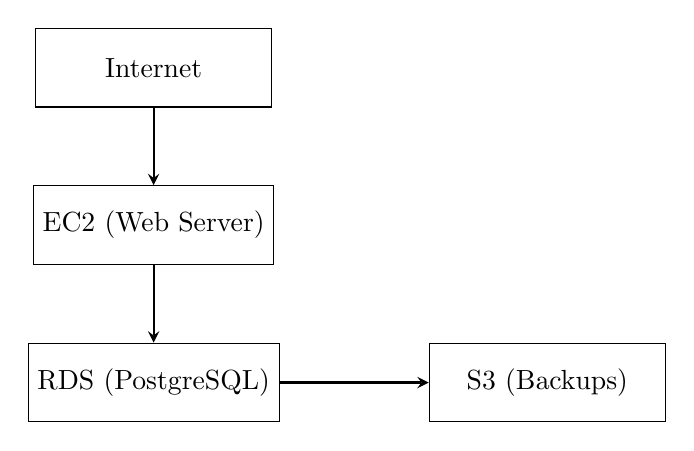
\begin{tikzpicture}[
    node distance=2cm,
    box/.style={rectangle, draw, minimum width=3cm, minimum height=1cm, text centered},
    arrow/.style={->, >=stealth, thick}
]
    \node[box] (internet) {Internet};
    \node[box, below of=internet] (ec2) {EC2 (Web Server)};
    \node[box, below of=ec2] (rds) {RDS (PostgreSQL)};
    \node[box, right of=rds, xshift=3cm] (s3) {S3 (Backups)};
    
    \draw[arrow] (internet) -- (ec2);
    \draw[arrow] (ec2) -- (rds);
    \draw[arrow] (rds) -- (s3);
\end{tikzpicture}
\end{center}

\subsection{AWS Services}

\textbf{Amazon RDS (Relational Database Service)}
\begin{itemize}
    \item Database PostgreSQL được quản lý tự động
    \item Instance: db.t3.micro (1 vCPU, 1GB RAM)
    \item Tự động backup, patch, monitoring
\end{itemize}

\textbf{Amazon S3 (Simple Storage Service)}
\begin{itemize}
    \item Lưu trữ backup database
    \item Durability: 99.999999999\%
    \item Encryption: AES-256
\end{itemize}

\textbf{Amazon EC2 (Elastic Compute Cloud)}
\begin{itemize}
    \item Máy chủ chạy ứng dụng
    \item Instance: t2.micro (1 vCPU, 1GB RAM)
\end{itemize}

\textbf{AWS IAM (Identity and Access Management)}
\begin{itemize}
    \item Quản lý quyền truy cập giữa EC2 và S3
\end{itemize}

\section{BACKUP \& RECOVERY}

\subsection{Công nghệ}

\textbf{PostgreSQL Tools}
\begin{itemize}
    \item \texttt{pg\_dump}: Export database thành file SQL
    \item \texttt{psql}: Import file SQL vào database
\end{itemize}

\textbf{AWS S3 + SDK}
\begin{itemize}
    \item Upload/download backup files
    \item Versioning enabled (tránh mất dữ liệu)
    \item Lifecycle policy tự động xóa backup cũ
\end{itemize}

\subsection{Backup Strategy - 3-2-1 Rule}

\textbf{3 copies:}
\begin{itemize}
    \item Original: Database trên RDS
    \item Backup 1: File local trên EC2
    \item Backup 2: File trên S3 cloud
\end{itemize}

\textbf{2 media:}
\begin{itemize}
    \item Local storage (EC2 disk)
    \item Cloud storage (S3)
\end{itemize}

\textbf{1 offsite:}
\begin{itemize}
    \item S3 bucket ở region khác (Singapore)
\end{itemize}

\subsection{Retention Policy}

\begin{itemize}
    \item Daily backups: Giữ 7 ngày
    \item Weekly backups: Giữ 4 tuần
    \item Monthly backups: Giữ 12 tháng
\end{itemize}

\subsection{Tự động hóa}

\begin{itemize}
    \item Task Scheduler (Windows) / Cron (Linux)
    \item Backup tự động 2:00 AM hàng ngày
    \item Tự động xóa backup cũ theo retention policy
\end{itemize}

\section{DEPLOYMENT}

\subsection{Tổng quan}

\textbf{EC2 Instance}
\begin{itemize}
    \item Chạy Nginx (web server) + Node.js (backend)
    \item PM2 process manager (auto-restart, monitoring)
    \item Kết nối RDS qua SSL/TLS
\end{itemize}

\textbf{RDS Database}
\begin{itemize}
    \item PostgreSQL 15/16
    \item Private subnet (không public access)
    \item Automated daily backups
\end{itemize}

\textbf{S3 Storage}
\begin{itemize}
    \item Lưu trữ backup files
    \item Chi phí: < \$1/tháng
\end{itemize}

\section{KẾT LUẬN}

\textbf{Reliability:} RDS automated backups, S3 durability 99.999999999\%

\textbf{Scalability:} Dễ dàng scale database và storage


\end{document}
